\documentclass[10pt,a4paper]{article}

\usepackage[
  top=1.2cm,
  bottom=1.2cm,
  left=1.2cm,
  right=1.2cm
]{geometry}
\usepackage{xcolor}
\usepackage{fontspec}
\usepackage{graphicx}
\usepackage{tabularx}
\usepackage{array}
\usepackage{enumitem}
\usepackage{hyperref}
\usepackage{setspace}

\pagestyle{empty}
\setlength{\parindent}{0pt}
\setlength{\parskip}{0pt}
\setstretch{1.03}

\definecolor{accent}{HTML}{1F4E79}
\definecolor{accent2}{HTML}{B23A48}
\definecolor{sidebg}{HTML}{F2F5F8}
\definecolor{textgray}{HTML}{555555}
\definecolor{rulegray}{HTML}{D7DDE4}
\definecolor{dark}{HTML}{1F2933}
\pagecolor{white}

\IfFontExistsTF{Songti SC}{
  \setmainfont{Songti SC}
}{
  \IfFontExistsTF{STSong}{
    \setmainfont{STSong}
  }{
    \setmainfont{Arial Unicode MS}
  }
}

\hypersetup{
  colorlinks=true,
  urlcolor=accent,
  linkcolor=accent,
  pdftitle={李培楠简历}
}

\setlist[itemize]{
  leftmargin=1.15em,
  itemsep=0.18em,
  topsep=0.18em,
  parsep=0pt
}

\newcommand{\sectionline}{\vspace{-0.55em}\color{rulegray}\rule{\linewidth}{0.8pt}\vspace{0.35em}}
\newcommand{\cvsection}[1]{%
  \vspace{0.55em}%
  {\Large\bfseries\color{accent}#1}\par
  \sectionline
}
\newcommand{\job}[4]{%
  \textbf{#1}\hfill \textcolor{textgray}{#2}\par
  \textit{#3}\hfill \textcolor{textgray}{#4}\par
}
\newcommand{\smallentry}[2]{%
  \textbf{#1}\hfill \textcolor{textgray}{#2}\par
}
\newcommand{\sidehead}[1]{%
  \vspace{0.45em}{\large\bfseries\color{dark}#1}\par
  \vspace{0.2em}\color{rulegray}\rule{\linewidth}{0.8pt}\vspace{0.35em}
}
\newcommand{\field}[2]{\textbf{#1} #2\par}

\begin{document}

\noindent
\begin{minipage}[t]{0.255\textwidth}
\colorbox{sidebg}{%
  \begin{minipage}[t]{\dimexpr0.255\textwidth-2\fboxsep\relax}
  \vspace{0.2em}
  \centering
  {\fontsize{23}{26}\selectfont\bfseries 李培楠}\par
  \vspace{0.4em}
  {\color{accent}\bfseries 同济大学}\par
  {\color{dark}机械工程与机器人学院}\par
  {\color{dark}机械制造及其自动化 2023级}\par
  {\color{textgray}本科生}\par

  \vspace{0.75em}
  \setlength{\fboxsep}{0.06cm}
  \setlength{\fboxrule}{0.5pt}
  \fcolorbox{rulegray}{white}{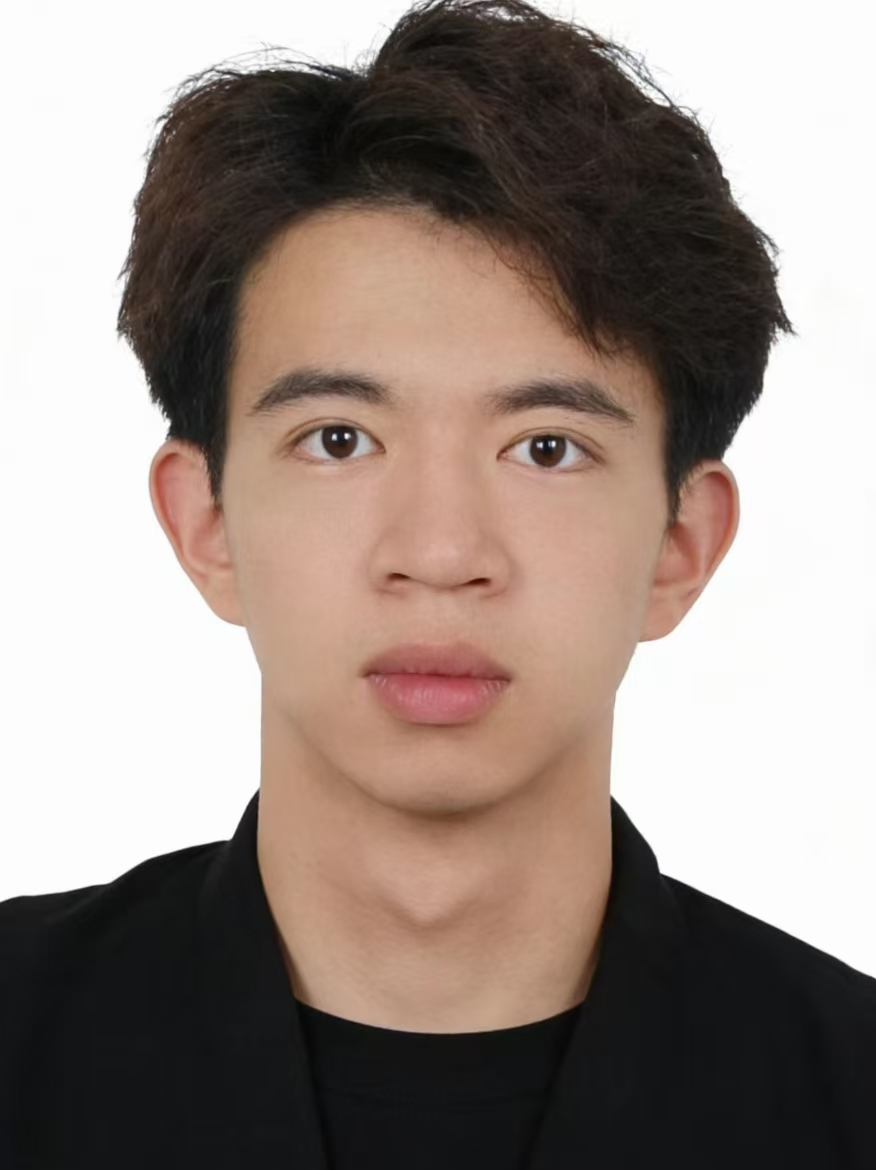
\includegraphics[width=0.70\linewidth]{证件照.jpg}}\par

  \vspace{0.75em}
  \sidehead{联系方式}
  \field{邮箱}{\href{mailto:19829058377@163.com}{19829058377@163.com}}
  \field{电话}{19829058377}
  \field{主页}{\href{https://peinanli.com}{peinanli.com}}
  \field{地点}{上海 / 广州}

  \sidehead{技能}
  \begin{itemize}
    \item Python, C/C++, Matlab
    \item ROS, Linux, Git
    \item 建模, 控制, 仿真, 数据分析
    \item LaTeX, 英文技术写作
  \end{itemize}

  \sidehead{语言}
  \begin{itemize}
    \item 英语能力：待补充
    \item 其他：待补充
  \end{itemize}
  \vspace{0.15em}
  \end{minipage}%
}
\end{minipage}\hfill
\begin{minipage}[t]{0.72\textwidth}
\vspace{0pt}

\cvsection{申请概述}
\textcolor{textgray}{同济大学机械工程与机器人学院机械制造及其自动化 2023 级本科生。此处建议补充你面向港科广红鸟硕士的研究兴趣、学术动机与核心优势，用 2--3 句概括即可。}

\cvsection{教育背景}
\job{同济大学，机械工程与机器人学院}{2023.09 -- 至今}{机械制造及其自动化，本科}{上海}
\begin{itemize}
  \item 核心课程：高等数学、线性代数、工程力学、机械设计、自动控制原理、机器人学、程序设计等
  \item 成绩排名：GPA / 专业排名 / 重要课程成绩，待补充
  \item 研究兴趣：机器人、智能制造、具身智能、控制与优化等方向
\end{itemize}

\cvsection{科研经历}
\job{课题 / 论文 / 实验室经历}{起止时间}{导师 / 团队 / 机构名称}{地点}
\begin{itemize}
  \item 用一句话说明研究问题、你的职责和采用的方法，例如建模、算法实现、实验设计、数据分析。
  \item 突出量化结果：性能提升、实验规模、论文、专利、报告、开源代码或展示成果。
\end{itemize}

\job{课题 / 论文 / 实验室经历}{起止时间}{导师 / 团队 / 机构名称}{地点}
\begin{itemize}
  \item 后续你给我内容后，我会把这里改成更像申请材料的表达。
\end{itemize}

\cvsection{项目经历}
\job{项目名称}{起止时间}{角色：负责人 / 核心成员 \quad 技术栈：Python / C++ / ROS / Matlab}{}
\begin{itemize}
  \item 说明项目目标、系统架构、你负责的模块，以及与机器人、智能制造或 AI 相关的技术细节。
  \item 给出结果：完成原型、仿真验证、实机测试、指标提升、竞赛名次或展示链接。
\end{itemize}

\job{项目名称}{起止时间}{角色：负责人 / 核心成员}{}
\begin{itemize}
  \item 建议每段项目经历控制在 2--4 条 bullet，重点写行动和结果。
\end{itemize}

\cvsection{荣誉奖项与竞赛}
\smallentry{奖项 / 竞赛名称}{获奖时间}
\begin{itemize}
  \item 奖项级别、排名或入选比例，若与申请方向相关可补充项目主题。
\end{itemize}
\smallentry{奖学金 / 荣誉称号}{获奖时间}
\begin{itemize}
  \item 例如校级 / 院级奖学金、优秀学生、科创竞赛等。
\end{itemize}

\cvsection{其他经历}
\smallentry{学生工作 / 志愿服务 / 社团经历}{起止时间}
\begin{itemize}
  \item 只保留能体现领导力、沟通协作或长期投入的经历；如果空间紧张可删去本模块。
\end{itemize}

\end{minipage}
\end{document}
